% Created 2023-07-21 Fri 22:00
% Intended LaTeX compiler: xelatex
\documentclass[hidelinks, 11pt]{article}
\usepackage{graphicx}
\usepackage{longtable}
\usepackage{wrapfig}
\usepackage{rotating}
\usepackage[normalem]{ulem}
\usepackage[leqno]{amsmath}
\usepackage{amssymb}
\usepackage{capt-of}
\usepackage{hyperref}
\usepackage{mathtools}
\usepackage{physics}
\usepackage[paperwidth=164mm, paperheight=232mm, left=20mm, right=20mm, top=20mm, bottom=20mm]{geometry}
\usepackage{enumerate}
\usepackage{multirow}
\usepackage{libertinust1math}
\usepackage{xepersian}
\settextfont{Yas}
\setlatintextfont{Linux Libertine}
\linespread{1.2}
\author{علیرضا عظیمی‌نیا $401\,205\,061$ \\ کیانا عسگری $97\,100\,473$}
\date{}
\title{\lr{Optimal Stopping via Randomized Neural Networks}}
\hypersetup{
 pdfauthor={},
 pdftitle={\lr{Optimal Stopping via Randomized Neural Networks}},
 pdfkeywords={},
 pdfsubject={},
 pdfcreator={Emacs 29.0.92 (Org mode 9.6.6)}, 
 pdflang={}}
\usepackage{biblatex}
\addbibresource{/home/alireza/org/biblio.bib}
\begin{document}

\maketitle

\section{مقدمه}
\label{sec:org43aa378}

چالش پیدا کردن بهترین زمان برای توقف یک فرایند به منظور بیشینه‌کردن
پاداش یا کمینه‌کردن هزینه، به مسئله یافتن زمان توقف بهینه
(\lr{optimal stopping time}) معروف است.  این مسئله یکی از
پرکاربردترین مسائل در آمار، اقتصاد و ریاضیات مالی است.  با وجود
اینکه الگوریتم‌های کنونی برای این مسئله مانند برنامه‌نویسی پویا
(\lr{dynamic programming}) یا استفاده از یادگیری تقویتی
(\lr{reinforcement learning}) عملکرد خوبی از خود نشان داده‌اند، اما در
ابعاد بالا عملکرد خوبی ندارند.

یکی از مهم‌ترین کاربردهای مسئله‌ی توقف بهینه در پیدا کردن بهترین زمان
اجرای یک قرارداد اختیار آمریکایی (\lr{American option}) است.
مقاله‌ی اصلی، دو الگوریتم بر مبنای شبکه‌های عصبی برای حل مسئله توقف بهینه
معرفی می‌کنند که تنها پارامترهای لایه آخر آن‌ها یاد گرفته می‌شوند.  ثابت
نگه داشتن پارامترهای پنهان در طول فرایند آموزش مسئله‌ی بهینه‌سازی را از
حالت غیر محدب به حالت محدب تبدیل می‌کند.  توابع پنهان در شبکه می‌توانند
نقش توابع پایه‌ای در رگرسیون را بازی کنند.  مقاله‌ی اصلی در ادامه،
الگوریتم‌های خود را به صورت خاص برای تعیین قیمت قراردادهای اختیار
آمریکایی تشریح می‌کند.

\section{تاریخچه}
\label{sec:orgfb561e4}

دو ایده‌ی معروف برای حل مسئله‌ی توقف بهینه، استقرای بازگشتی یا به عبارتی
برنامه ریزی پویا
\LTRfootnote{J. N. Tsitsiklis and B. Van Roy. Regression methods for pricing complex american-style options. IEEE Transactions on Neural Networks, 12(4), 2001.}
و استفاده از یادگیری تقویتی
\LTRfootnote{J. N. Tsitsiklis and B. Van Roy. Optimal stopping of markov processes: Hilbert space theory, approximation algorithms, and an application to pricing high-dimensional financial derivatives. IEEE Transactions on Automatic Control, 44(10), 1999.}
است.  هر دوی این روش‌ها، بر اساس تخمین کمترین مربعات هستند و نیاز به
انتخاب مجموعه‌ای از توابع پایه دارند.  علاوه بر اینکه انتخاب این مجموعه
دشوار است، با افزایش ابعاد مسئله تعداد توابع پایه مورد نیاز به صورت چند
جمله‌ای یا نمایی افزایش می‌یابد که استفاده از این ایده‌ها را در ابعاد بالا
غیرممکن می‌سازد.

ایده‌ای نسبتاً جدید، استفاده از شبکه‌های عصبی به عنوان جایگزین توابع پایه
است.  شبکه‌های عصبی در فضای توابع \(L^{p}(\mu)\) برای \(1\leq p<\infty\)
و اندازه متناهی \(\mu\) چگال هستند و در اکثر مسائل به نفرین ابعاد
(\lr{curse of dimensionality}) دچار نمی‌شوند.  در مقابل، شبکه‌های عصبی
توابع غیرمحدبی هستند و روش‌های بر پایه‌ی کاهش گرادیان لزوماً به مینیمم
سراسری همگرا نخواهند بود.

مقاله‌ی اصلی تلاش می‌کند هم به مشکل نفرین ابعاد و هم به مشکل همگرایی
اثبات‌پذیر غلبه کند.

\section{قرارداد اختیار خرید آمریکایی}
\label{sec:org9685929}

چنین قراردادی به دارنده‌ی قرارداد اختیار خرید یک دارایی با قیمتی معین را
در هر لحظه‌ای تا زمان سررسید می‌دهد.  چنین قراردادی را می‌توان با یک
قرارداد برمودان (\lr{Bermudan Option}) تخمین زد؛ به این شکل که دارنده‌ی
قرارداد تنها امکان اجرای آن را در زمان‌های گسسته \(t_0<t_1<\cdots<t_N\)
خواهد داشت.  تعیین قیمت این نوع قراردادها یکی از کاربردهای مسئله‌ی توقف
بهینه است.

فرض می‌کنیم عایدی (\lr{payoff}) قراداد که آن را با \(g\) نشان می‌دهیم تنها
به قیمت فعلی سهام بستگی دارد: \(g=g(X_{t})\).  به عنوان مثال
\(g(X)=\max\{0,X-K\}\).

فرض می‌کنیم \((X_{t})_{t\geq 0}\) یک فرایند مارکوف باشد که قیمت سهام‌ها را
توصیف می‌کند.  چنین فرایندی می‌تواند توسط یک معادله دیفرانسیل، مانند
مدل \lr{Black-Scholes}، توصیف شود:
\begin{align*}
	dX_{t} & = X_{t} (r\, dt + \sigma \,dW_{t}), \\
	X_{0}  & = x_{0}
\end{align*}
معادله بالا یک حرکت براونی هندسی را توصیف می‌کند:
\begin{equation*}
  X_{t} = x_{0} \exp \left[ \left(\mu-\frac{\sigma^{2}}{2}\right)t
    + \sigma W_{t} \right]
\end{equation*}

تقریبی گسسته از قرارداد اختیار خرید آمریکایی در نظر می‌گیریم: بازه‌ی زمانی
\([0,T]\) را به \(N\) قسمت مساوی تقسیم می‌کنیم، و برای سادگی، زمان‌ها را
با \(0,1,\dots,N\) نشان می‌دهیم.  در این صورت، قیمت قرارداد اختیار خرید
در زمان \(n\) بصورت زیر است:
\begin{equation*}
	U_{n} = \sup_{t\geq n} E\left(\alpha^{t-n} g(X_{t}) \;\middle|\; X_{n}\right)
\end{equation*}
که \(\alpha\) نرخ تعدیل است.  معادلاً
\begin{equation}
  \label{U:price}
  \begin{split}
	U_{N} & = g(X_{N}), \\
	U_{n} & =
	  \max \big\{ g(X_{n}), E(\alpha U_{n+1} \mid X_{n}) \big\},
	    \quad  0\leq n < N
  \end{split}
\end{equation}

در هر لحظه، عایدی قرارداد \(g(X_{n})\) در آن لحظه با مقدار
\(c_{n}(X_{n})=E(\alpha U_{n+1} \mid X_{n})\) مقایسه می‌شود و بر اساس آن
زمان توقف بهینه \(\tau_{n}\) با شروع از زمان \(n\) بدست می‌آید:
\begin{equation}
  \label{tau:optimal}
  \begin{split}
	‍\tau_{N} & = N, \\
	\tau_{n} & =
	   n \text{ \lr{if} } g(X_{n}) \geq c_{n}(X_{n}),
	   \text{ \lr{otherwise} } \tau_{n} = \tau_{n+1}
  \end{split}
\end{equation}
به خصوص
\begin{equation*}
	U_{0} =
	  \max \Big\{
	     g(X_{0}), E \big( \alpha^{\tau_{1}} g(X_{\tau_{1}}) \big)
	  \Big\}
\end{equation*}

\section{شبیه‌سازی \lr{Monte Carlo}}
\label{sec:org596406b}

فرض می‌کنیم روشی برای شبیه‌سازی \(X_{t}\) داریم.  هر شبیه‌سازی یک مسیر از
قیمت سهام‌ها با شروع از \(x_{0}\) می‌دهد.  \(m\) بار قیمت سهام‌ها را
شبیه‌سازی می‌کنیم و آنها را به صورت \(x_{0},x_{1}^{i},\dots,x_{N}^{i}\)
نشان می‌دهیم.  اندیس بالا برای مسیر، و اندیس پایین برای زمان است.  با
توجه به (\ref{U:price}) اگر استراتژی توقف (\ref{tau:optimal}) را دنبال
کنیم، جریان نقدی که نصیبمان می‌شود برابر است با
\begin{equation}
  \label{p:price}
  \begin{split}
	p_{N}^{i} & = g(x_{N}^{i}), \\
	p_{n}^{i} & =
	  g(x_{n}^{i}) \text{ \lr{if} } g(x_{n}^{i}) \geq c_{n}(x_{n}^{i}),
	  \text{ \lr{otherwise} } p_{n}^{i} = \alpha p_{n+1}^{i}
  \end{split}
\end{equation}
به عبارتی دیگر، \(\{p_{n}^{i}\}_{i=1}^{m}\) نمونه‌هایی از
\(\alpha^{\tau_{n}-n}g(X_{n})\) هستند و می‌توان از آنها برای تقریب
\(U_{n}\) استفاده کرد.  به خصوص با توجه به قانون اعداد بزرگ می‌توان نوشت:
\begin{equation}
	\label{U0:price}
	U_{0} \approx
	  \max \Big\{
	     g(x_{0}), \frac{1}{m} \sum_{1}^{m} \alpha p_{1}^{i}
	  \Big\}
\end{equation}

\section{تقریب توابع \(c_{n}\) با استفاده از شبکه عصبی}
\label{sec:org86c574b}

در هر زمان \(n\)، مقدار \(c_{n}(x)\) برابر میانگین قیمت تعدیل‌شده قرارداد
\(\alpha U_{n+1}\) است در صورتی که قیمت فعلی سهام‌ها \(x\) باشد و قرارداد
را تا زمان \(n+1\) اجرا نکنیم.

برای تقریب هر کدام از \(c_{n}\)ها از یک شبکه عصبی دولایه که فقط پارامترهای
لایه‌ی آخر یادگرفته شدند استفاده می‌کنیم. (شکل)

\begin{figure}[htbp]
  \centering
  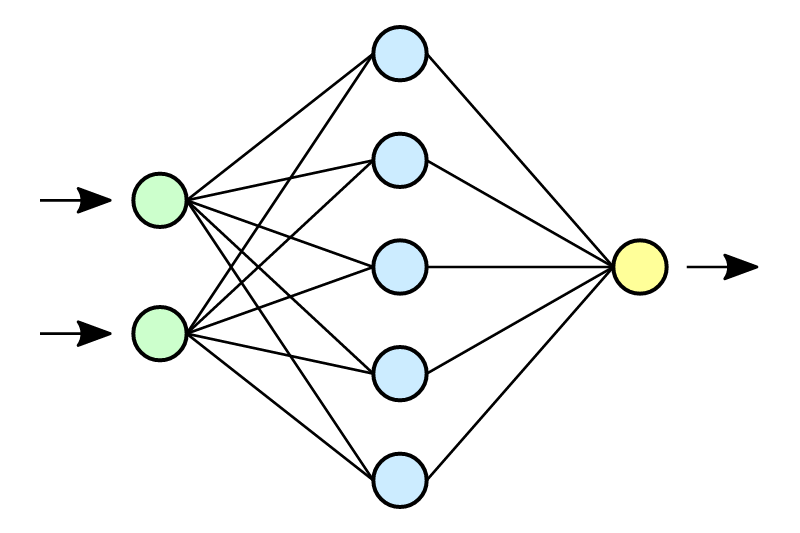
\includegraphics[scale=0.3]{Neural_network.png}
\end{figure}

تابع فعال‌سازی (\lr{activation function}) را با \(\sigma\) نشان
می‌دهیم. مثلاً \lr{leaky ReLU}:
\begin{equation*}
	\sigma(x)=\max(0,x)-\max(0,-ax)
\end{equation*}
فرض کنید \(d\) سهام به عنوان ورودی و \(k\) گره در لایه میانی داشته
باشیم.  ماتریس \(A\in\mathbb{R}^{k\times d}\) و بردار
\(b\in\mathbb{R}^{k}\) که وزن‌ها و بایاس لایه‌ی اول هستند را بصورت تصادفی
انتخاب می‌کنیم.  \(A,b\) برای تمام \(c_{n}\)ها مشترک است.  برای هر
\(c_{n}\)، بردار \(A_{n}\in\mathbb{R}^{k}\) و عدد \(b_{n}\in\mathbb{R}\)
که وزن و بایاس لایه‌ی آخر هستند باید یاد گرفته شوند.  اکنون تقریبی از
\(c_{n}\) که با \(\widetilde{c}_{n}\) نشان می‌دهیم در دسترس است:
\begin{equation}
	\label{c:nn}
	\widetilde{c}_{n}(x) = A_{n} \cdot \sigma (Ax+b) + b_{n}
\end{equation}
از طرفی \(c_{n}(x_{n}^{i})=\alpha p_{n+1}^{i}\).  پس \(A_{n}\) و
\(b_{n}\) بهینه از طریق حل مسئله رگرسیون خطی
\begin{equation}
	\label{mc:reg}
	A_{n} \cdot \sigma (Ax_{n}^{i}+b) + b_{n}
	  \approx \alpha p_{n+1}^{i},    \quad i=1,\dots,m
\end{equation}
بدست می‌آیند.  برای این کار، می‌توان از روش مینیمم‌کردن خطای کمترین مربعات
استفاده کرد:
\begin{equation*}
	\mathrm{MSE} =
	  \frac{1}{m} \sum_{1}^{m}
	     \left( \widetilde{c}_{n}(x_{n}^{i})-\alpha p_{n+1}^{i} \right)^{2}
\end{equation*}

از آنجایی که \(p_{N}^{i}\) مشخص است، با حل (\ref{mc:reg}) می‌توان
\(A_{N-1}\) و \(b_{N-1}\) بهینه را پیدا کرد.  اکنون با محاسبه
\(\widetilde{c}_{N-1}\) از (\ref{c:nn}) با توجه به (\ref{p:price})
می‌توان \(p_{N-1}^{i}\) را حساب کرد.  سپس از آن می‌توان برای محاسبه
\(\widetilde{c}_{N-2}\) و \(p_{N-2}^{i}\) استفاده کرد.  به همین ترتیب به
شکل بازگشتی می‌توان \(p_{n}^{i}\) را برای هر زمانی حساب کرد.  در نهایت با
داشتن \(p_{1}^{i}\)ها، از رابطه‌ی (\ref{U0:price}) می‌توان تقریبی از قیمت
قرارداد در لحظه صفر بدست آورد.

\section{تقریب توابع \(c_{n}\) با یادگیری تقویتی}
\label{sec:orge1595a7}

در قسمت قبل، هر تابع \(c_{n}\) را مجزا تقریب زدیم و از \(N-1\) شبکه عصبی
برای این کار استفاده کردیم.  در این قسمت از یک شبکه عصبی برای تقریب همه‌ی
\(c_{n}\)ها استفاده می‌کنیم.  چنین تقریبی فرمی مشابه (\ref{c:nn}) دارد:
\begin{equation}
	\label{c:rl}
	\widetilde{c}(n,x) =
	   \widetilde{A} \cdot \sigma (A\widetilde{x}+b) + \widetilde{b}
\end{equation}
که \(A\in\mathbb{R}^{k\times(d+2)}\) و \(b\in\mathbb{R}^{k}\) پارامترهای
لایه‌ی اول هستند که به طور تصادفی انتخاب می‌شوند،
\(\widetilde{x}=(n,N-n;x)\) برداری به طول \(d+2\) است، و
\(\widetilde{A}\) و \(\widetilde{b}\) مانند قسمت قبل پارامترهای لایه‌ی
آخر هستند و به طور بهینه انتخاب می‌شوند.  برای آموزش چنین شبکه‌ای از روش
\lr{Q-learning} استفاده می‌کنیم.

فرض کنید \(\pi\) یک استراتژی توقف باشد.  تابع ارزش برای این استراتژی به
صورت زیر است:
\begin{align*}
  Q^{\pi}(t, X_{t};\text{stop})
  &= g(X_{t}) \\
  Q^{\pi}(t, X_{t};\text{cont})
  &= \alpha\, \sum_{a\in\{\text{stop},\text{cont}\}}
      \pi(a\mid t+1,X_{t+1})\; Q^{\pi}(t+1,X_{t+1};a)
\end{align*}
برای استراتژی بهینه (\ref{tau:optimal})، داریم:
\begin{align}
  \label{Q:optimal}
  Q^{\ast}(t, X_{t};\text{stop})
  &= g(X_{t}) \nonumber \\
  Q^{\ast}(t, X_{t};\text{cont})
  &= \alpha\, \max_{a\in\{\text{stop},\text{cont}\}}Q^{\ast}(t+1,X_{t+1};a)
\end{align}
در زمان \(N\) اکشن \(\text{cont}\) غیرمجاز است.  در هر وضعیت
\((t,X_{t})\)
 با مقایسه‌ی دو مقدار \(Q^{\ast}(t, X_{t};\text{stop})\) و
\(Q^{\ast}(t, X_{t};\text{cont})\) اکشن بهینه در آن وضعیت مشخص می‌شود.
چون \(Q^{\ast}\) تابع ارزش استراتژی توقف بهینه (\ref{tau:optimal}) بود،
نتیجه می‌شود: \(Q^{\ast}(n,X_{n};\text{cont})=c_{n}(X_{n})\).  برای تقریب
\(Q^{\ast}\) از تابعی به فرم (\ref{c:rl}) استفاده می‌کنیم.

با یک حدس اولیه \(\widetilde{c}_{0}\) شروع کنید.  با داشتن
\(\widetilde{c}_{j}\)، برای \(i\in\{1,\dots,m\}\) و زمان
\(n\in\{1,\dots,N-1\}\) قرار دهید:
\begin{equation*}
	p_{n}^{i} = \max \left\{\widetilde{c}_{j}(n,x_{n}^{i}), g(x_{n}^{i})\right\}
\end{equation*}
توجه کنید که \(p_{N}^{i}=g(x_{N}^{i})\).  اکنون از روش مینیمم‌کردن خطای
کمترین مربعات، \(\widetilde{c}_{j+1}\) را تعیین کنید:
\begin{equation*}
	\mathrm{MSE} =
	  \frac{1}{m N} \sum_{n=1}^{N-1} \sum_{i=1}^{m}
	     \left( \widetilde{c}_{j}(n, x_{n}^{i})-\alpha p_{n+1}^{i} \right)^{2}
\end{equation*}
می‌توان ثابت کرد
\LTRfootnote{John Tsitsiklis and Benjamin Van Roy. Regression methods for pricing complex american-style options. IEEE Transactions on Neural Networks, 12(4):694–703, 2001. Section 6}
که دنباله \(\widetilde{c}_{j}\) همگراست به تقریبی بهینه
به فرم (\ref{c:rl}).  اکنون می‌توان از (\ref{p:price}) و
(\ref{U0:price}) قیمت قرارداد را در زمان صفر حساب کرد.

\section{الگوریتم}
\label{sec:orgc543956}

تعداد \(2m\) مسیر از فرایند تصادفی \(X_{t}\) شبیه‌سازی می‌کنیم.
در تاریخ سررسید، قیمت قرارداد برابر عایدی آن است:
\(p_{N}^{i}=g(x_{N}^{i})\).

در الگوریتم بازگشتی \lr{Monte Carlo}، ابتدا با استفاده از \(m\) مسیر اول
و روشی که در بخش مربوطه توضیح داده شد، توابع \(\widetilde{c}_{n}\) را
بدست می‌آوریم.  سپس با استفاده از \(m\) مسیر دوم و رابطه
(\ref{U0:price}) قیمت تقریبی قرارداد را در زمان صفر حساب می‌کنیم.

صورت کامل این الگوریتم،
\lr{randomized least squares Monte Carlo (RLSM)}:

\begin{enumerate}[1:]
\item

 ماتریس \(A\in\mathbb{R}^{k\times d}\) و بردار \(b\in\mathbb{R}^{k}\)
  را به طور تصادفی تولید کنید.

\item

 تعداد \(2m\) مسیر از فرایند تصادفی \(X_{t}\) (قیمت سهام‌ها در طول زمان)
  تولید کنید: \(x_{1}^{i},\dots,x_{N}^{i}\)

\item

 برای هر مسیر \(i\in\{1,\dots,2m\}\) قرار دهید: \(p_{N}^{i}=g(x_{N}^{i})\).

\item

 برای هر زمان \(n\in\{N-1,\dots,1\}\):

  \begin{enumerate}[a:]
  \item

 برای هر مسیر \(i\in\{1,\dots,2m\}\) قرار دهید:
    \(\phi(x_{n}^{i})=(\sigma(Ax_{n}^{i}+b),1)\in\mathbb{R}^{k+1}\)

  \item

  جواب مسئله کمترین مربعات
  \begin{equation*}
  	\sum_{i=1}^{m} \left(\phi(x_{n}^{i}) \cdot x - \alpha p_{n+1}^{i}\right)^{2}
  \end{equation*}
  را \(\theta_{n}\) بنامید: \(\theta_{n}\in\mathbb{R}^{k+1}\).

  \item

 برای هر مسیر \(i\in\{1,\dots,2m\}\): اگر
    \(g(x_{n}^{i})\geq\theta_{n}\cdot\phi(x_{n}^{i})\)، آنگاه قرار دهید
    \(p_{n}^{i}=g(x_{n}^{i})\)، در غیر این صورت قرار دهید
    \(p_{n}^{i}=\alpha p_{n+1}\).
  \end{enumerate}

\item

 قرار دهید \(p_{0}=\max\left\{g(x_{0}),m^{-1}\sum_{m+1}^{2m}\alpha p_{1}^{i}\right\}\).

\end{enumerate}

روند مشابهی را برای الگوریتم یادگیری تقویتی در پیش می‌گیریم.   با استفاده
از \(m\) مسیر اول پارامترهای تابع \(\widetilde{c}\) را تقریب می‌زنیم، سپس
با \(m\) مسیر دوم قیمت اولیه قرارداد را محاسبه می‌کنیم.

صورت کامل این الگوریتم،
\lr{randomized fitted Q-iteration (RFQI)}:

\begin{enumerate}[1:]
\item


 ماتریس \(A\in\mathbb{R}^{k\times(d+2)}\) و بردار \(b\in\mathbb{R}^{k}\)
  را به طور تصادفی تولید کنید.

\item

 تعداد \(2m\) مسیر از فرایند تصادفی \(X_{t}\) تولید کنید.

\item

قرار دهید \(\theta_{0}=0\in\mathbb{R}^{k+1}\) , \(j=0\).

\item

 تا همگرایی \(\theta_{j}\) فرایند زیر را تکرار کنید:

   \begin{enumerate}[a:]
   \item

  برای هر مسیر \(i\in\{1,\dots,2m\}\) قرار دهید:
  \(p_{N}^{i}=g(x_{N}^{i})\).

   \item

   برای هر زمان \(n\in\{1,\dots,N-1\}\) و هر مسیر \(i\in\{1,\dots,2m\}\)
   قرار دهید:
   \begin{align*}
     & \phi(n,x_{n}^{i})
      = \left(\sigma(A\widetilde{x}_{n}^{i}+b), 1\right) \in \mathbb{R}^{k+1}  \\
     & p_{n}^{i}
      = \max \left\{ g(x_{n}^{i}), \phi(n,x_{n}^{i})\cdot\theta_{j} \right\}
   \end{align*}
   که \(\widetilde{x}_{n}^{i}=(n,N-n;x_{n}^{i})\).

   \item

   جواب مسئله کمترین مربعات
   \begin{equation*}
     \sum_{n=1}^{N-1} \sum_{i=1}^{m}
     \left( \phi(n, x_{n}^{i}) \cdot x - \alpha p_{n+1}^{i} \right)^{2}
   \end{equation*}
   را \(\theta_{j}\) بنامید: \(\theta_{j}\in\mathbb{R}^{k+1}\).

   \item

   قرار دهید: \(j\leftarrow j+1\)

   \end{enumerate}

\item

از روی
\begin{align*}
  p_{N}^{i} & = g(x_{N}^{i}), \\
  p_{n}^{i} & =
    g(x_{n}^{i}) \text{ \lr{if} } g(x_{n}^{i}) \geq \phi(n,x_{n}^{i})\cdot\theta,
    \text{ \lr{otherwise} } p_{n}^{i} = \alpha p_{n+1}^{i}
\end{align*}
مقادیر \(p_{1}^{i}\) را حساب کنید.

\item

قرار دهید \(p_{0}=\max\left\{g(x_{0}),m^{-1}\sum_{m+1}^{2m}\alpha p_{1}^{i}\right\}\).


\end{enumerate}


\section{شبیه‌سازی}
\label{sec:org98ac9a9}

کد پیاده‌سازی الگوریتم‌های بالا در فایل \texttt{simulation.py} قرار دارد.
در پیاده‌سازی و شبیه‌سازی این الگوریتم‌ها ملاحظات زیر در دستور کار بوده است:

\begin{itemize}
\item از مدل \lr{Black-Scholes} برای شبیه‌سازی \(X_{t}\) استفاده شده است.
برای تولید یک مسیر \(X_{t}\) از الگوریتم زیر استفاده کردیم:

\begin{enumerate}[1:]
\item گام زمانی \(dt\) را به شکل مناسب انتخاب کنید: \(dt=T/N\).
\item بردارهای تصادفی \(Z_{t}\in\mathbb{R}^{d}\)، \(t=1,\dots,N\)، که
  عناصر آن‌ها از توزیع استاندارد نرمال آمده‌اند تولید کنید.
\item برای هر \(t=1,\dots,N\) قرار دهید
  \begin{equation*}
    X_{t} = x_{0} \prod_{i=1}^{t}
    \exp \left(
      \left( \mu - \frac{\sigma^{2}}{2} \right) dt + \sigma\, \sqrt{dt}\; Z_{i}
    \right)
  \end{equation*}
  منظور این است که عبارت بالا را درایه به درایه برای \(Z_{i}\) حساب
  کنید و حاصل را که یه بردار با ابعادی برابر ابعاد \(Z_{t}\) است
  \(X_{t}\) بنامید.
\end{enumerate}

\item درایه‌های ماتریس \(A\) و بردار \(b\) به صورت تصادفی از توزیع استاندارد
نرمال انتخاب شده‌اند.

\item تابع عایدی همان \(g(x)=(\max(x_{1},\dots,x_{d})-K)_{+}\) است به ازای
\(K=100\).

\item تابع فعال‌سازی \lr{leaky ReLU} است: \(\sigma(x)=\max(0,x)-\max(0,-ax)\)
به ازای \(a=0.5\).

\item هایپرپارامترهای الگوریتم به این شکل انتخاب شده‌اند: \(T=1\)، \(N=10\)،
\(m=10\,000\)، \(k=20\)، \(\alpha=1\)، \(\mu=0\)، \(\sigma=0.2\).
\item تعداد سهام‌ها \(d\) از بین \(\{5,10,50,100,500,1\,000\}\)، و قیمت اولیه
سهام‌ها \(x_{0}\) از بین مقادیر \(\{80,100,120\}\) انتخاب شده‌اند.
\end{itemize}


نتایج شبیه‌سازی‌ها در دو جدول زیر آمده است.  می‌توان دید که اعداد بدست آمده
بسیار به نتایج شبیه‌سازی مقاله‌ی اصلی نزدیک است.

\begin{latin}
\begin{table}[htbp]
\centering
\begin{tabular}{|cc|r|r|}
\cline{3-4}
\multicolumn{2}{}{}         &            \multicolumn{2}{|c|}{price}                  \\ \hline
d                   & $x_0$ & \multicolumn{1}{|c|}{RLSM} & \multicolumn{1}{|c|}{RFQI} \\ \hline
                    & 80    & 4.64   ( 0.13 )            & 4.98   ( 0.06 )            \\
5                   & 100   & 23.94  ( 0.20 )            & 24.53  ( 0.09 )            \\
                    & 120   & 48.32  ( 0.21 )            & 49.25  ( 0.33 )            \\ \hline
                    & 80    & 8.24   ( 0.08 )            & 8.81   ( 0.08 )            \\
10                  & 100   & 32.81  ( 0.16 )            & 33.61  ( 0.14 )            \\
                    & 120   & 59.30  ( 0.13 )            & 60.36  ( 0.17 )            \\ \hline
                    & 80    & 21.81  ( 0.06 )            & 22.84  ( 0.07 )            \\
50                  & 100   & 52.26  ( 0.09 )            & 53.51  ( 0.13 )            \\
                    & 120   & 82.76  ( 0.11 )            & 84.12  ( 0.17 )            \\ \hline
                    & 80    & 28.40  ( 0.08 )            & 29.26  ( 0.05 )            \\
100                 & 100   & 60.47  ( 0.08 )            & 61.6   ( 0.08 )            \\
                    & 120   & 92.57  ( 0.15 )            & 93.81  ( 0.19 )            \\ \hline
                    & 80    & 43.07  ( 0.06 )            & 43.64  ( 0.07 )            \\
500                 & 100   & 78.81  ( 0.10 )            & 79.55  ( 0.12 )            \\
                    & 120   & 114.55 ( 0.08 )            & 115.42 ( 0.15 )            \\ \hline
                    & 80    & 49.12  ( 0.09 )            & 49.63  ( 0.05 )            \\
1000                & 100   & 86.37  ( 0.06 )            & 87.05  ( 0.11 )            \\
                    & 120   & 123.66 ( 0.12 )            & 124.42 ( 0.14 )            \\ \hline
\end{tabular}
\caption{Max call option on Black–Scholes for different number of stocks $d$ and varying initial stock price $x_0$.}
\end{table}
\end{latin}

\begin{latin}
\begin{table}[htbp]
\centering
\begin{tabular}{|cc|r|r|}
\cline{3-4}
\multicolumn{2}{}{}         &            \multicolumn{2}{|c|}{price}                     \\ \hline
d                   & $N$   & \multicolumn{1}{|c|}{RLSM} & \multicolumn{1}{|c|}{RFQI}    \\ \hline
                    & 10    & 32.73 ( 0.14 )             & 33.63 ( 0.20 )                \\
10                  & 50    & 31.54 ( 0.17 )             & 34.05 ( 0.13 )                \\
                    & 100   & 31.04 ( 0.22 )             & 34.23 ( 0.12 )                \\ \hline
                    & 10    & 52.28 ( 0.09 )             & 53.57 ( 0.11 )                \\
50                  & 50    & 50.62 ( 0.10 )             & 53.88 ( 0.14 )                \\
                    & 100   & 50.15 ( 0.11 )             & 54.01 ( 0.10 )                \\ \hline
                    & 10    & 60.55 ( 0.08 )             & 61.59 ( 0.11 )                \\
100                 & 50    & 58.77 ( 0.07 )             & 61.93 ( 0.14 )                \\
                    & 100   & 58.26 ( 0.09 )             & 62.06 ( 0.15 )                \\ \hline
\end{tabular}
\caption{Max call option on Black–Scholes for different number of stocks $d$ and higher number of exercise dates $N$.}
\end{table}
\end{latin}

\section{نتایج}
\label{sec:orgf706b32}

مقاله‌ی اصلی مقایسه‌ی وسیعی بین دو الگوریتم \lr{RLSM} و \lr{RFQI} و
الگوریتم‌های مشابه این حوزه از حیث سرعت اجرا و دقت قیمت خروجی انجام داده
است.  گزاره‌های زیر را مستقیم از مقاله اصلی نقل می‌کنیم:

\begin{latin}
  \begin{quote}
    In all cases RLSM and RFQI are the fastest algorithms while
    achieving at least similar prices to the best performing
    baselines. Their biggest strength are high dimensional problems
    \(d\geq 500\), where this speed-up becomes substantial.

    In these high dimensional problems, RLSM outperforms all baselines
    in terms of prices, even tough RLSM has much less trainable
    parameters.  RFQI achieves the highest prices there, and therefore
    works best, while having considerably less trainable parameters.

    RLSM and RFQI are considerably faster than existing algorithms for
    high dimensional problems.  For high dimensions \(d\geq 500\), RLSM
    is about 8 times faster than the fastest baseline NLSM (Neural Least
    Square Monte Carlo) and about 30 times faster than DOS (Deep Optimal
    Stopping).

    RLSM and RFQI are up to 2400 (and 4800) times faster than LSM (and
    FQI respectively) with basis functions of order 2, 5 to 16 times
    faster than NLSM and 20 to 66 times faster than DOS.

    When increasing the number of exercise dates for the maxcall option
    on Black–Scholes from \(N=10\) to \(N\in\{50,100\}\) the Bermudan
    option price should become closer to the American option price.
    RFQI is more than 30 times faster than DOS for high dimensions.
    Increasing the number of dates further, the computation time can
    become a limiting factor for DOS, while this is not the case for
    RFQI.
  \end{quote}
\end{latin}

‬\pagebreak

در مورد مقایسه بین دو الگوریتم \lr{RLSM} و \lr{RFQI}:

\begin{latin}
  \begin{quote}
    Reinforcement learning techniques usually outperform the backward
    induction in the Markovian setting.  RFQI, achieving similar prices
    as FQI, therefore naturally outperforms RLSM which achieves similar
    prices as LSM.

    A possible explanation for the outperformance of the reinforcement
    learning algorithm is the following: The backward induction
    algorithms have approximately \(N\) times the number of trainable
    parameters used in the reinforcement learning algorithms, since a
    different network is trained for each discretisation date.
    Moreover, for the backward induction algorithms, a different
    continuation value function is approximated for each date, hence,
    only the data of this date is used to learn the parameters.  In
    contrast, the reinforcement learning methods train their parameters
    using the data of all dates.  Hence, the reinforcement learning
    methods use \(N\) times the number of data to train \(1/N\) times
    the number of parameters, which seems to lead to better
    approximations.
  \end{quote}
\end{latin}
\end{document}